\documentclass[12pt]{extarticle}

\setlength{\headheight}{16pt} % ??? we do what fancyhdr tells us to do  

\title{Mathematical Modelling for ML}
\author{Giacomo Ellero}
\date{a.y. 2024/2025}

\usepackage{preamble}

%\renewcommand{\vec}[1]{\uvec{#1}}
\renewcommand{\vec}[1]{\bm{#1}}

\begin{document}

\oldfirstpage

\section{Introduction}

Assume our data is of the form $(x_n, y_n)$, where $x \in \R ^d$ and $y \in \R$
and we want to find a predictor $f_\theta(\cdot): \R^d \to \R$.

To figure out how good our model is we want to find a \emph{loss function} which tells us
how far is our predicted value from the real one.
Ideally we'd like to \say{count} the errors we make and use that as our loss function,
however these functions are usually not differentiable.
To fix this problem we look for another function which is differentiable and bounds the \say{true}
loss function, an example is the \emph{square error} (as we saw in statistics).
Eventually we want to find a model which minimizes the average loss:
\begin{equation}
	\argmin_\theta \bm R_\text{emp}(\theta) = \frac{1}{N} \sum_{i = 1}^N \ell(y_i, \hat y_i)
\end{equation}
Note that we will use $\theta$ and $w$ interchangeably,
they both represents the parameters/coefficients/weights of our model.

As we saw in linear regressions, the best estimator for $w$ is
\begin{equation}
	\hat w= (W^T W)^{-1} X^T y
\end{equation}
However, the Hessian matrix (given by $\laplacian \ell (w) = X^T X$)
is \emph{positive semi-definite}: this means that the function indeed has a global minimum,
but it might not be unique.
If we find more than one minimum we take the one which is closer to the origin:
in this way we avoid noise as much as possible.

\subsection{Reducing overfitting}
When we train our model we try to minimize the error against the training set.
Then we run the model against the test dataset:
of course we will get a higher loss than on the training set, however we want to check how the model
behaves when we modify the number of parameters to check for overfitting or underfitting.

\begin{figure}[H]
	\centering
	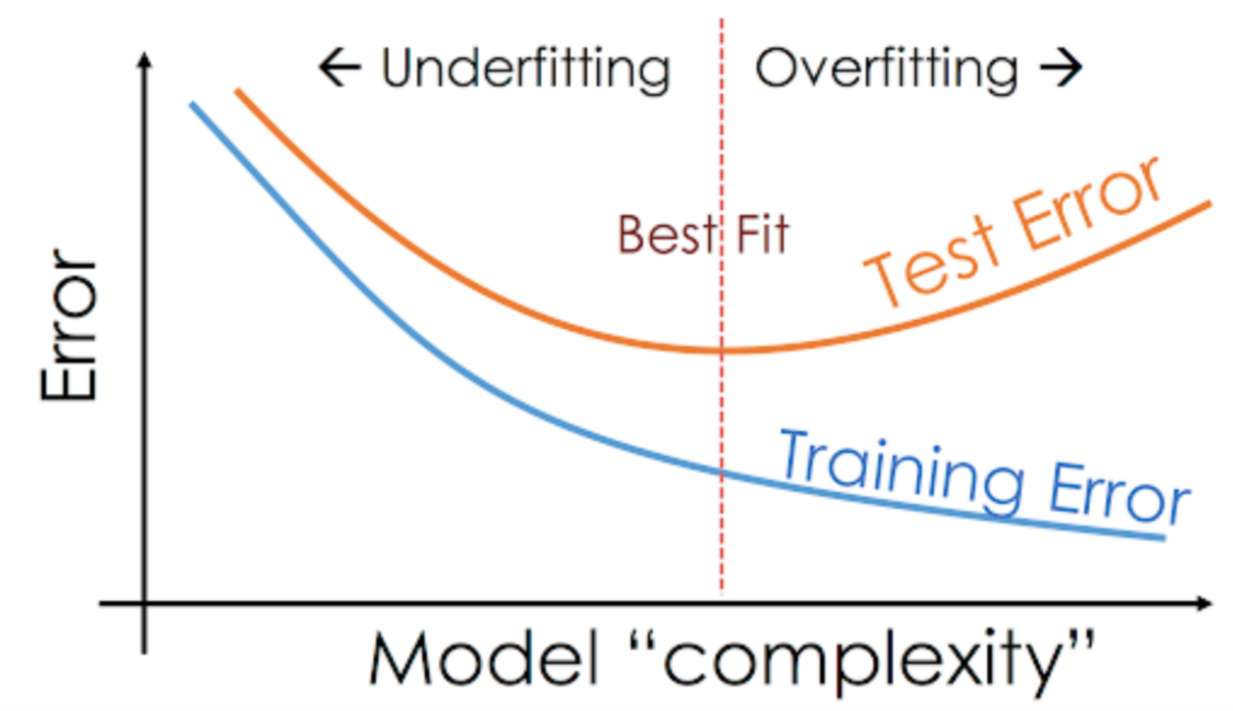
\includegraphics[width=0.5\textwidth]{./assets/modelling-ml/overfitting-vs-underfitting.jpg}
	\caption{Graph of the loss function as the number of parameters changes.}
\end{figure}

To reduce the number of parameters and ensure positive definiteness (i.e. uniqueness of the minimum)
we can use a \emph{Ridge regression} (see statistics), where we penalize the model based on the
magnitude of the parameters, this is more numerically stable.

\subsection{Bayes theorem}

\begin{equation}
	p(\theta \mid x) = \frac{p(x\mid \theta) p(\theta)}{p(x)}
\end{equation}

Our final goal is to compute the posterior $p(\theta \mid x)$.
This is hard by itself, however by using the theorem we can separate it in \say{computable}
chunks: $p(x \mid \theta)$ is the easiest; while the prior $p(\theta)$
is definitely more \say{guessable}.

Instead of minimizing the negative maximum likelihood estimator
we minimize the negative log-posterior
using a technique called \emph{maximum a posteriori} estimation.
\begin{equation}
	\argmin_\theta - \log [p(x \mid \theta) p(\theta)]
\end{equation}

\subsection{Kullback-Leibler divergence}

The definition of the KL divergence is
\begin{equation}
	D_{KL}(p,q) = \sum_{x \in X} p(x) \log \frac{p(x)}{q(x)}
\end{equation}
This is a way to measure the distance between two functions.
We can use this to minimize the distance between the given data and some theoretical distribution.
We can model the empirical data into an actual distribution by considering its histogram:
this distribution will just be a sum of $\delta$ functions of the observations we had.

\begin{proposition}{Non-negativity of DL-divergence}{dl-non-neg}
	For all probability measures $p, q$ we have that $D_{KL}(p, q) \geq 0$.
\end{proposition}

\begin{proof}
	First invert the sign of the definition:
	\begin{align}
		-D_{KL}(p,q)          & = -\sum_{x \in X} p(x) \log \frac{p(x)}{q(x)}   \\
		                      & = \sum_{x \in X} p(x) \log \frac{q(x)}{p(x)}    \\
		                      & \leq \log \sum_{x \in X} p(x) \frac{q(x)}{p(x)} \\
		                      & = \log \sum_{x \in X} q(x)                      \\
		                      & = \log (1) = 0                                  \\
		\implies D_{KL}(p, q) & \geq 0
	\end{align}
	where we have used Jensen inequality.
\end{proof}

\subsubsection{KL divergence and MLE}

He proved that they are basically the same thing but
I think he'll go over this again in the next class.

TODO: FINISH HERE

\section{Perceptron}

This is a model that tries to work similarly to the actual biological neurons.
The simplest model of a neuron looks like
\begin{equation}
	y = \Theta \left(\sum_i w_i x_i - T \right)
\end{equation}
where $y \in \{0, 1\}$ is the neuron output (either it fires or it doesn't),
$\Theta$ is the Heavisde function defined as
\begin{equation}
	\Theta(x) = \begin{cases}
		1 & \text{if } x \geq 0 \\
		0 & \text{otherwise}
	\end{cases}
\end{equation}
while $w_i$ are called weights and $x_i$ are the outputs of other connected neurons.
$T$ is the fire threshold.

By changing the weight we can modify the way that neurons fire: this is a phenomenon which happens
also in biological brains.

Depending on how the neurons are connected to each other we can define \emph{feedforward}
networks, where each neuron is connected only to some \say{next} ones, and \emph{recurrent} ones,
where we can have neurons which link back to other neurons, this for example allows for short-term.

\subsection{Learning}

There are multiple way an actor can learn: we can have an unsupervised learning where the actor
is just trying to make statistical sense of the input;
we can have reinforced learning where the actor gets a reward for a correct output, this is what
happens with dopamine in biological brain;
we can have supervised learning where the actor knows what it wants to achieve and it gets feedback
on how good or bad it did, for example trying to throw a ball at a target.

\begin{figure}[H]
	\centering
	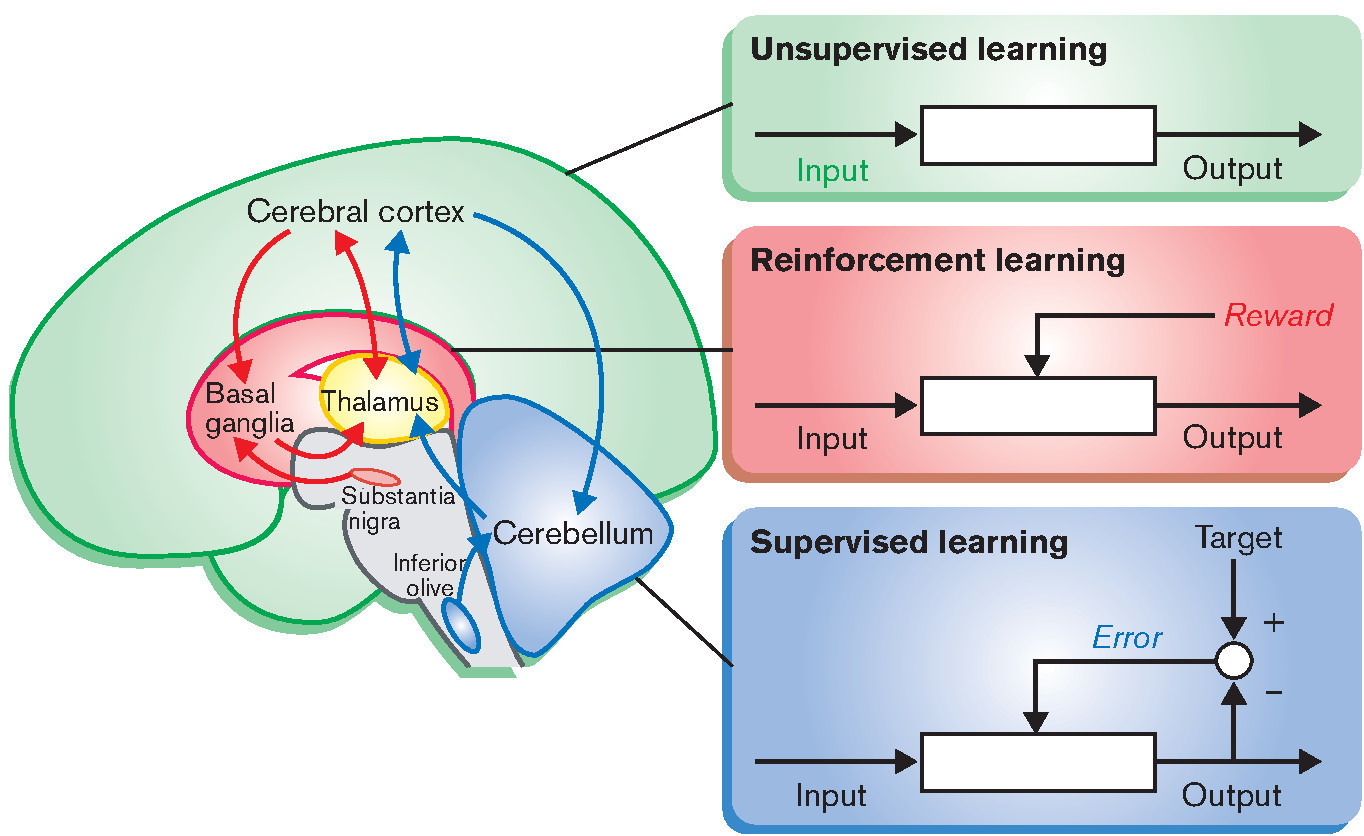
\includegraphics[width=0.5\textwidth]{./assets/modelling-ml/brain-learning-types.jpg}
	\caption{Different parts of the brain learn in different modes.}
\end{figure}

We want our model to be able to classify inputs $\vec x^\mu$ as $y^\mu \in \{0, 1\}$,
that is, we want to find some weights $\vec w$ such that
\begin{equation}
	y^\mu = \Theta(\vec w \cdot \vec x^\mu)
\end{equation}
Geometrically, this is equivalent to finding an hyperplane which divides the two sets of inputs.

A simple perceptron is able to solve problems where the inputs are already linearly separable,
for more complex inputs we will need to add hidden layers, but we will cover this further
ahead in the course.

\subsubsection{Learning algorithm}

Initialize $t = 0$ and $\vec w_t$.
Now iterate on $t$: pick a pattern $\mu$, if $\vec w_t$ gives the right output we leave it the same,
if it doesn't we modify $\vec w_{t+1}$ as follows
\begin{equation}
	\vec w_{t + 1} = \begin{cases}
		\vec w_t + \eta \vec x^\mu & \text{if } y^mu = 1 \\
		\vec w_t - \eta \vec x^\mu & \text{if } y^mu = 0
	\end{cases}
\end{equation}
where $\eta \in \R$ is the learning rate.

\begin{proposition}{Convergence of the perceptron algorithm}{perceptron-convergence}
	If there exists an hyperplane which separates the inputs as desired
	the perceptron algorithm will converge to it.
\end{proposition}

\begin{proof}
	Let $\vec z^\mu = (2 y^\mu - 1) \vec x^mu$.
	We assume that $\exists K : \norm{\vec z^\mu} < K$.

	Then
	\begin{equation}
		\vec z^\mu = \begin{cases}
			\vec x^\mu  & \text{if }y^\mu = 1 \\
			-\vec x^\mu & \text{if }y^\mu = 0
		\end{cases}
	\end{equation}
	such that $\vec w \cdot \vec z^\mu > 0$.

	We claim that if there exists $\vec w^*$ such that $\norm{\vec w^*} = 1$ and
	$\vec w^* \cdot \vec z^\mu > \varepsilon$ for all $\mu$ the algorithm will converge.

	The idea of this claim is that we want to find a lower bound for $A_t = \vec w_t \cdot \vec w^*$
	and an upper bound for $B_t = \norm{\vec w^*}$.
	Assume there exists a $\mu$ such that such $\vec w^*$ exists and $\vec w_t \cdot \vec z^\mu <0$,
	now we do the $t+1$ modification.

	TODO: finish here
\end{proof}

\subsubsection{Capacity of a perceptron}
Given a set of $p$ associations $\vec x^\mu \to y^\mu$ what is the probability to find
a weight vector that correctly classifies all input patterns?

We know perceptrons can only work for patterns which are separable by an hyperplane.
Therefore our task is to find the probability that our inputs can be separated by a hyperplane.

We solve this problem geometrically, by finding the number of dichotomies of the input (that is,
what are the possible ways we can color the inputs with two colors).
In particular we look for \emph{linear dichotomies}, which are the patterns in which we can separate
the two colors with an hyperplane.

\begin{proposition}{Probability of finding a linear dichotomy}{prob-lin-dichotomy}
	The probability of finding a linear dichotomy in a set of $p$ points in $N$ dimensions is
	\begin{equation}
		P = \frac{1}{2^{p-1}} \sum_{k = 0}^{N -1} \binom{p-1}{k}
		\label{eq:prob-lin-dichotomy}
	\end{equation}
\end{proposition}

\begin{proof}
	Let $C(p, N)$ be our goal function which counts the number of linear dichotomies of $p$ points
	in $N$ dimensions.

	We know that the total number of dichotomies is $2^p$, which means that the probability of finding
	a linear dichotomy is
	\begin{equation}
		P = \frac{C(p, N)}{2^p}
	\end{equation}

	Suppose we know $C(p, N)$ and we add another point: we want to compute $C(p + 1, N)$.
	To do so we count the ways we can move the separating hyperplane without changing the output
	of the other $p$ points, but this is equivalent to counting the linear dichotomies where
	the separating hyperplane goes through a particular point.
	Since now we are constraint by passing through a point the number of dimensions
	is reduced to $N-1$, therefore we conclude that
	\begin{equation}
		C(p+1, N) = C(p, N) + C(p, N-1)
	\end{equation}

	Now we check that \cref{eq:prob-lin-dichotomy} is correct.
	Recall the way we construct Pascal's triangle: there holds that
	\begin{equation}
		\binom{p}{k} = \binom{p-1}{k} + \binom{p-1}{k-1}
	\end{equation}
	We know that $C(1, N) = 2$ and since $\binom{0}{0} = 1$ we have $C(1, N) = 2 \binom{0}{0}$.
	Then
	\begin{align}
		C(p+1, N) & = 2 \sum_{k = 1}^{N-1} \binom{p}{k}                                           \\
		          & = 2 \sum_{k = 1}^{N-1} \binom{p-1}{k} + 2 \sum_{k = 1}^{N-1} \binom{p-1}{k-1} \\
		          & = C(p, N) + 2 \sum_{k = 1}^{N-2} \binom{p-1}{k}                               \\
		          & = C(p, N) + C(p, N-1)
	\end{align}
	where we have shifted the sum by one in the third step.
\end{proof}

We can study what happens in the limit:
\begin{itemize}
	\item $p \leq N \implies P = 1$;
	\item $N \leq p \leq 2N \implies P \to 1$ as $N \to \infty$;
	\item $p = 2N \implies P = 0.5$
	\item $p > 2N \implies P \to 0$ as $N\to \infty$.
\end{itemize}
We notice that we have a very sharp bound at $p = 2N$ which separates the cases where $P = 0$ and
the ones where $P = 1$. We call $p = 2N$ the \emph{capacity} of the perceptron.

\subsubsection{Continuous perceptron}
If $y^\mu$ is a continuous variable, instead of being in $\{0, 1\}$, we need to define a cost
function $\phi$ such that

NEXT CLASS!

\end{document}
